\begin{figure}[H]
\centering
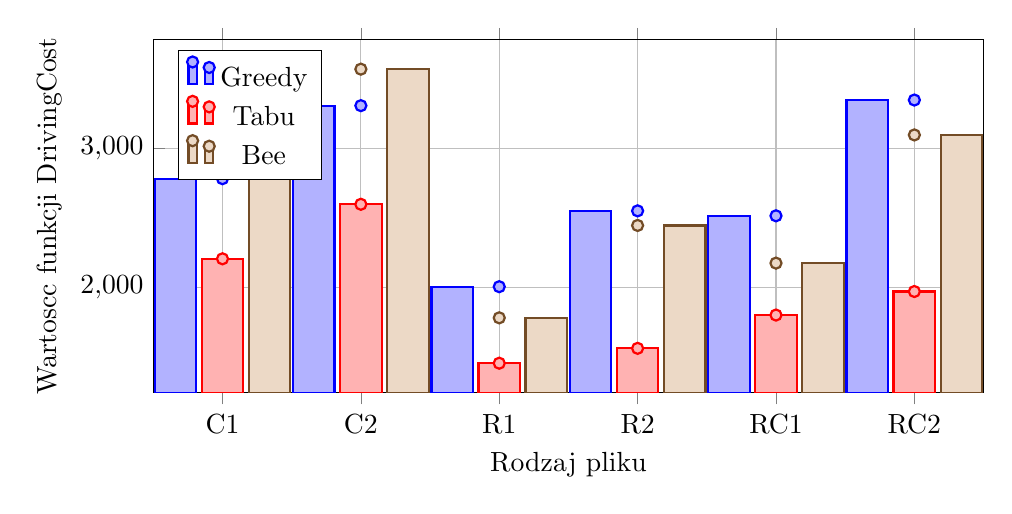
\begin{tikzpicture}
\begin{axis}[
xlabel = {Rodzaj pliku},
ylabel = {Wartoscc funkcji DrivingCost},
legend pos = north west,
grid = both,
width=1\linewidth,
height=0.5\linewidth,
ybar,
bar width=15pt,
symbolic x coords={C1,C2,R1,R2,RC1,RC2,},
xtick=data
]
\addplot + [mark = *, thick] coordinates
    {
(C1,2783.222222222222)(C2,3309.375)(R1,2004.9166666666667)(R2,2551.3636363636365)(RC1,2515.75)(RC2,3350.0)};
\addlegendentry
{Greedy}
\addplot + [mark = *, thick] coordinates
    {
(C1,2205.8888888888887)(C2,2598.75)(R1,1453.6666666666667)(R2,1560.8181818181818)(RC1,1800.625)(RC2,1970.25)};
\addlegendentry
{Tabu}
\addplot + [mark = *, thick] coordinates
    {
(C1,2932.222222222222)(C2,3572.375)(R1,1780.5454545454545)(R2,2446.2727272727275)(RC1,2174.75)(RC2,3098.5)};
\addlegendentry
{Bee}
\end{axis}
\end{tikzpicture}
\caption
{Porownanie srednich wartosci DrivingCost algorytmow dla kazdego rodzaju pliku}
\label{fig:mean_DrivingCost_comparision}
\end{figure}
